\documentclass[12pt,fleqn]{article}
\setlength{\parindent}{0pt}
\usepackage{graphicx}
\usepackage{cancel}
\usepackage{listings}
\usepackage[latin5]{inputenc}
\usepackage{color}
\setlength{\parskip}{8pt}
\setlength{\parsep}{0pt}
\setlength{\headsep}{0pt}
\setlength{\topskip}{0pt}
\setlength{\topmargin}{0pt}
\setlength{\topsep}{0pt}
\setlength{\partopsep}{0pt}
\setlength{\mathindent}{0cm}
\usepackage{latexsym}
\usepackage{amsfonts}
\usepackage{mathrsfs}
\usepackage{showkeys}
\renewcommand*\showkeyslabelformat[1]{(#1)}

\begin{document}
Ders 4

Disbukeylik (Convexity) ve Koniler (Cones)

Bir lineer vektor uzayindaki $K$ kumesi disbukeydir (convex), eger 
$x_1,x_2
\in K$ icin $\alpha x_1 + (1-\alpha)x_2$, $0 \le \alpha \le 1$ formundaki
tum noktalar da $K$ icinde ise.

Matematiksel olarak $\alpha,1-\alpha$ ile yapilmaya ugrasilan $x_1,x_2$
``arasindaki'' bir noktayi temsil etmek. Eger $0 \le \alpha \le 1$ ise,
$x_1,x_2$'yi sirasiyla $\alpha,1-\alpha$ ile carpip sonuclari toplamak
``biraz $x_1$'den, biraz $x_2$'den almak'' anlamina geliyor, bu da tanim
itibariyle her zaman $x_1,x_2$ arasinda bir yerde olmaktir. 

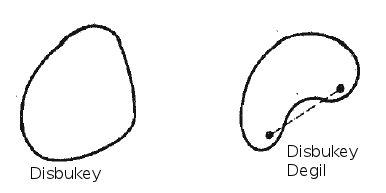
\includegraphics[height=3cm]{4_1.png}

Ve eger bu ``arada olmak'' denklemi, kumedeki her noktanin her diger
noktayla arasindaki, yani her $\alpha$ icin hesaplanacak noktalar icin de
dogru ise, o zaman hep ayni kumedeyi, ``disari cikmiyoruz'' demektir ve bu
disbukeyligin tanimidir. Gorsel olarak ta kabaca bunu gormek mumkundur,
disbukey bir cisimde bir noktadan digerine duz cizgide giderken hep cisim
icinde kaliriz.

Teori 

$K.G$ bir vektor uzayinda disbukey olan iki kume olsun. O zaman 

1. $\alpha K = \{x: x = \alpha k, k \in K\}$ her $\alpha$ icin disbukeydir. 

2. $K+G$ disbukeydir. 

Ispatlamadan bunun daha genel bir hali olan baska bir teoriye bakalim, onu
ispatlarsak usttekini de ispatlamis olacagiz. 

Teori 

$\mathscr{C}$, icindeki tum kumeleri disbukey olan rasgele bir buket
olsun. O zaman $\cap_{K \in \mathscr{C}}K$ ayni sekilde disbukeydir. 

Ispat

Diyelim ki $C = \cap_{K \in \mathscr{C}}K$. Eger $C$ bos ise, teori hemen
ispatlamistir. Diger sartlar icin, farzedelim ki $x_1,x_2 \in C$. O zaman
$x_1,x_2 \in K$ demektir, cunku $C$ bir kesisim, yani tum $K \in \mathscr{C}$
icindeki ayni olan ogelerden mutesekkil. Her $K$'nin kendi basina disbukey
oldugunu bildigimize gore, o zaman $C$ de disbukey demektir. 

\[ \square \]

Norm Edilmis Lineer Uzaylar

Soyut Analiz ve uygulamalarda ilgilenilen vektor uzaylarinin 7 onsarttan
daha fazlasina ihtiyaci vardir. 7 onsart vektor uzaylarinin sadece cebirsel
ozelliklerini tanimlar: toplam, skalar carpim, ve bunlarin degisik
kombinasyonlari. Eksik olanlar topolojik olan ozelliklerdir, yani aciklik
(openness), kapalilik (closure), yaklasiksallik (convergence), ve butunluk
(completeness). Eger uzayin icinde uzaklik olcumu tanimlanir ise, bu
kavramlar kullanilabilir. 

Tanim

Norm edilmis bir lineer uzay $X$ adindaki bir vektor uzayidir, ki $X$
icindeki her $x$ ogesini bir reel sayi $||x||$'e esleyen bir fonksiyon
vardir, ve $||x||$'e $x$'in norm'u adi verilir. Norm su onsartlari yerine
getirmelidir. 

1. $||x|| > 0$, her $x \in X$ icin, ve $||x|| = 0$, sadece ve sadece $x =
\theta$ ise. 

2. $||x+y|| \le ||x|| + ||y||$ her $x,y \in X$ icin (ucgensel esitsizlik) 

3. $||\alpha x|| = |\alpha| \ ||x||$, her skalar $\alpha$ ve her $x \in X$ icin. 

Norm kavrami uzaklik kavraminin soyutlastirilmis bir halinden ibaret
aslinda. Reel analizdeki ucgensel esitsizligin karsiligi burada da
goruluyor mesela. Neyse, devam edelim, ustteki ucgensel esitsizlik
kuralinin bir uzantisi / sonucu (lemma) su:

Teori 

Norm edilmis bir lineer uzayda $||x|| - ||y|| \le ||x-y||$. 

Ispat

\[ ||x|| - ||y|| = ||x - y + y|| - ||y||\]

Ustte adece $||x||$ icine $-y+y$ ekliyoruz, yani aslinda hicbir sey
degistirmedik. Simdi esitligin sagindaki ilk terimi alip ona ucgensel
esitligi uygularsak (norm icindeki $+$ isareti solu ve sagindaki gruplari
ayri terimler olarak kabul etmemiz gerekir)

\[ ||x - y + y|| - ||y|| \le
||x - y || + ||y|| - ||y|| 
\]

elde ederiz. Biraz daha basitlestirince

\[ ||x|| - ||y||  \le ||x - y ||  \]

$\square$

Uygun bir norm bulunabilirse, daha once gosterdigimiz vektor uzayi
orneklerinin cogunlugu norm edilebilen uzaya donusturulebilir.

Ornek 1

$C[a,b]$ adi verilen norm edilmis uzay, $[a,b]$ reel araligi, arti norm

\[ ||x|| = \min_{a \le t \le b} |x(t)| \]

tanimindan olusur. Bu uzay daha once bir vektor uzayi olarak
gosterilmisti. Simdi teklif edilen norm'un 3 gerekli onsarti yerine getirip
getirmedigine bakalim.










\end{document}
